\documentclass[t, notes, xcolor=table]{beamer}

\usepackage{wrapfig}
\usepackage{float}
% For tabs in verbatim
\usepackage{fancyvrb}

% Adjust position of the image
\usepackage[export]{adjustbox}

% set fonts
\usefonttheme{professionalfonts} % using non standard fonts for beamer
\usepackage{txfonts,mathptmx}

% set indend spacing for first and second level indentation
\setlength{\leftmargini}{0.5cm}
\setlength{\leftmarginii}{0.5cm}
\setlength{\leftmarginiii}{0.5cm}

% Set circles for bullets 
\setbeamertemplate{itemize items}[circle]

% colors
\usepackage{xcolor}

% multiple columns
\usepackage{multicol}

% todo lists
\usepackage{pifont}
\usepackage{amssymb}

% increase space between text and frame name
\addtobeamertemplate{frametitle}{}{\vspace{0.5em}}

%Information to be included in the title page:
\title{Choosing Between Verilog Data Types}
\author{Nikola Petrovic}
\institute{University of Belgrade, School of Electrical Engineering}
\date{2022}



\begin{document}

\frame{\titlepage}

%%%%%%%%%%%%%%%%%%%%%%%%%%%%%%%%%%%%%%%%%%%%%%%%%%%%%%%%%%%%
\begin{frame}
\frametitle{Module Objective}

In this module we will choose and use the Verilog data types correctly.
\newline

\textbf{Topics}

\begin{itemize}
\item Logic values
\item Net and Register type rules and example
\item Declaring vectors (truncation and padding)
\item Defining literal values
\item Declaring nets
\item Declaring variables
\item Declaring arrays of nets and variables
\item Declaring module parameters
\end{itemize}

\end{frame}

%%%%%%%%%%%%%%%%%%%%%%%%%%%%%%%%%%%%%%%%%%%%%%%%%%%%%%%%%%%%
\begin{frame}
\frametitle{Value Set}
\footnotesize{

\begin{tabular}{ |c|l| } 
\hline
 \rowcolor{lightgray} 
 Value & Associated Informal Terms  \\ 
 \hline
 0 & Zero, Low, False, Logic Low, Ground, VSS  \\ 
 \hline
 1 & One, High, True, Logic High, Power, VDD, VCC  \\ 
 \hline
 Z & HiZ, High Impedance, Tri-State, Undriven, Unconnected, Driver disabled   \\ 
 \hline
 X & Uninitialized, Unknown  \\ 
 \hline
\end{tabular}
}
\end{frame}

\note{

\footnotesize{
The Verilog value set consists of four basic values:
\begin{itemize}
\item 0 - Represents a logic zero, low, false condition
\item 1 - Represents a logic one, high, true condition
\item Z - Represents a high impedance state
\item X - Represents an unknown state
\end{itemize}
}
}

\note{

\tiny{
The simulator initializes most nets to high-impedance state. The exception are nets of \textbf{trireg} type, this is because they represents capacitive nets so they are initialized to unknown value.
\newline

Upon commencing the simulation, simulator propagates the values of net drivers onto the nets. A net that has no drivers will remain in its initialized value throughout the simulation. This situation is usually the result of user error, as there are seldom good reason to leave a net undriven.
\newline

The simulator initialized most variables to unknown value. The exception is variable of the \textbf{real} type, which is initialized to 0 since this is the only type that cannot hold high-impedance or unknown values.
\newline

A variable that is never assigned a value will remained in its initialized value throughout simulation.
\newline

The appearance during simulation of a high-impedance value on a net is usually due to its drivers being disabled. In real hardware this situation either has short duration or doesn't occur because bus keepers pull the nets to a high or a low logic states. 
\newline

The appearance during simulation of a unknown value on a net is usually due to clash between drivers driving different values. In real hardware, this situation will either not exist or have an extremely short duration.
\newline

The appearance during simulation of a high-impedance value on a variable is due to the assignment of that value to the variable, either deliberately because that value represents one of the drivers on the bus net, or by assigning a value of a net to a variable. 
\newline

The appearance during simulation of a unknown value on a variable is due to the assignment of that value to the variable, either deliberately because the simulator cannot resolve the value of assigned expression, or by assigning a value of a net to a variable. In real hardware, variable will assume 0 or 1 state.

}
}

%%%%%%%%%%%%%%%%%%%%%%%%%%%%%%%%%%%%%%%%%%%%%%%%%%%%%%%%%%%%
\begin{frame}
\frametitle{Data Types}

Verilog provides three groups of value objects and different types in each group:
\begin{itemize}
\item \textcolor{blue}{Nets}
\begin{itemize}
	\item Represents physical connection between structure and objects supply0, suppy1, tri\textbackslash wire, tri0, tri1, triand\textbackslash wand, trior\textbackslash wor, trireg
\end{itemize}
\item \textcolor{blue}{Variables}
\begin{itemize}
	\item Represents abstract storage elements: integer, real, reg, time, realtime 
\end{itemize}
\item \textcolor{blue}{Parameters}
\begin{itemize}
	\item Run-time constants: localparam, parameter, specparam
\end{itemize}
\end{itemize}
\end{frame}


\note{
\scriptsize{
Procedures communicate by passing events, and by passing data via nets and shared variables informally called signals. Verilog does not actually have things called signals. Verilog has three group of value objects and only a very few types in each group:
\begin{itemize}
\item Verilog has \textbf{nets} to represent physical connection between structure and objects (supply0, suppy1, tri\textbackslash wire, tri0, tri1, triand\textbackslash wand, trior\textbackslash wor, trireg).
\item It has \textbf{variables} to represent abstract storage elements (integer, real, reg, time, realtime).
\item Verilog has two simulation-time constants and a annotatable constant (localparam, parameter and specparam). These are constants and it is illegal to modify them run-time.
\end{itemize}
}
}
%%%%%%%%%%%%%%%%%%%%%%%%%%%%%%%%%%%%%%%%%%%%%%%%%%%%%%%%%%%%
\begin{frame}
\frametitle{Net and Register Type Rules}

We can specify the type upon declaration.
\begin{itemize}
\item \textcolor{blue}{Nets} and \textcolor{blue}{registers} are one-bit wide unless you also specify the range.
\item A port declaration implicitly declares an one-bit \textcolor{blue}{wire} net unless you explicitly declare otherwise.
\end{itemize}

Rules govern our use of data types:
\begin{itemize}
\item Variables can only be driven inside procedures.
\item Nets are driven everywhere else (outside procedures)
\item Constants are for unchanging or instance-specific values.
\end{itemize}

\end{frame}

\note{
\scriptsize{
A data item has associated with it the data values it can have and rules for how you use it.
\newline

A net is the recipient of its drivers' values.
\newline

A variable is an item you procedurally assign values to.
\newline

A port is a net or variables that the instantiating module can connect its own net or variables to.
\newline

A parameter is like a variable but has a constant value.
\newline

Ports, nets, and variables of the \textbf{reg} type are a single bit unless you declare them with a range.
\newline

These module headers show two ways to declare ports:
\begin{itemize}
\item We can list the ports in the module header and later declare them as a module item
\item As of the Verilog 2001 update, we can directly declare the ports in the module header.
\end{itemize}
}
}

%%%%%%%%%%%%%%%%%%%%%%%%%%%%%%%%%%%%%%%%%%%%%%%%%%%%%%%%%%%%
\begin{frame}
\frametitle{Type Rules in Connectivity}

\begin{itemize}
\item Module \textcolor{purple}{input} ports are always nets.
\item Module \textcolor{purple}{output} ports are variables if driven by a procedural block, or nets in all other cases.
\item Connections to the \textcolor{purple}{input} ports of a module instance are variables if driven by a procedural block,, or nets in all other cases.
\item Connections to the \textcolor{purple}{output} ports of a module instance are always nets.
\item Connections to bidirectional \textcolor{purple}{inout} ports are always nets.
\end{itemize}

\begin{figure}[H!]
    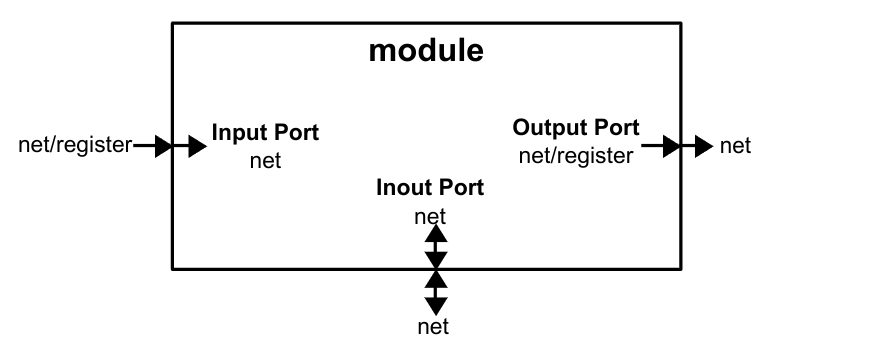
\includegraphics[width=0.7\textwidth]{img/04_nets.png}
\end{figure}

\note{
A port permits an external net or variable to connect to an internal net or variable, with restrictions.

Here are some common user errors, along with their typical error messages:
\begin{itemize}
\item We make a procedural assignment to a signal that we either declared as a net or we forgot to declare so is thus implicitly a net. This is an illegal statement.
\item We connect an output from an instance to a signal declared as a register. This is illegal as a module output can only drive a net. This is an illegal output port specification.
\item We declare a signal as a module input and as a register. This is illegal as inputs can only be nets. These are incompatible declarations.
\end{itemize}
}
\end{frame}


%%%%%%%%%%%%%%%%%%%%%%%%%%%%%%%%%%%%%%%%%%%%%%%%%%%%%%%%%%%%
\begin{frame}[fragile]
\frametitle{Net and Register Type Example}

\begin{multicols}{2}
{\tiny%
\begin{Verbatim}[commandchars=\\\{\}, tabsize=2]
\textcolor{purple}{module} yin(
	\textcolor{purple}{output reg} y_out,
	\textcolor{purple}{input wire} a_in, b_in
);
\textcolor{purple}{always} @ (a_in or b_in)
	y_out = a_in && b_in;
\textcolor{purple}{endmodule}

\textcolor{purple}{module} yang(
	\textcolor{purple}{output wire} y_out,
	\textcolor{purple}{input wire} a_in, b_in
);
\textcolor{purple}{assign} y_out <= a_in || b_in;
\textcolor{purple}{endmodule}

\textcolor{purple}{module} yin_and_yang_tb;
	\textcolor{purple}{reg} a, b;
	\textcolor{purple}{wire} and_out, or_out;
	yin u1 (and_out, a, b);
	yang u2 (or_out, a, b);
	\textcolor{purple}{initial begin}
		a = 0;
		b = 0;
		...
	\textcolor{purple}{end}
\textcolor{purple}{endmodule}
\end{Verbatim}
}

\vfill

\columnbreak

\begin{figure}[H!]
    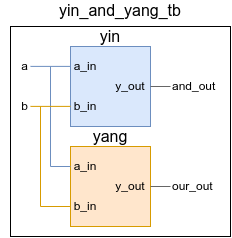
\includegraphics[width=0.45\textwidth]{img/04_net_example.png}
\end{figure}
\end{multicols}

\end{frame}

\note{
\scriptsize{
We are using here fully defined Verilog-2001 ANSI-C syntax for module port declarations for clarity.
\newline

In both module yin and yang, the input ports a\_in and b\_in \textbf{must} be declared as net data types.
\newline

In module yin, the output y\_out \textbf{must} be declared as a register data type as it is assigned from the \textit{always} procedural block.
\newline

In module yang, the output y\_out \textbf{must} be declared as a net type as it is driven from the continuous assign statement.
\newline

In module \textit{test}, a and b \textbf{must} be declared as register data types as they are assigned from the \textit{initial} procedural block, but and\_out and or\_out \textbf{must} be declared as net data types as they are driven from the instance output ports.
\newline

Therefore a connection like a -$>$ a\_in, or y\_out -$>$ and\_out actually changes data type as it crosses the module boundary.

}
}
%%%%%%%%%%%%%%%%%%%%%%%%%%%%%%%%%%%%%%%%%%%%%%%%%%%%%%%%%%%%
\begin{frame}[fragile]
\frametitle{Declaring Vectors}

A vector is a net or reg with a range specification.

We can specify the vector's range when declaring the variable:
\begin{itemize}
\item {[msb : lsb]} or {[lsb: msb]}
\item Range can be ascending or descending
\item Bounds can be negative, zero or positive
\item Bounds must be constant expressions
\item Individual bits can be selected from a vector
\end{itemize}

\begin{multicols}{2}
{\footnotesize%
\begin{Verbatim}[commandchars=\\\{\}, tabsize=2]
\textcolor{purple}{module} mux4 (
	\textcolor{purple}{input wire} [3:0] a, b,
	\textcolor{purple}{input wire}       sel,
	\textcolor{purple}{output reg} [3:0] op
);
\textcolor{purple}{always} @ (a or b or sel)
	\textcolor{purple}{if} (sel == 1)
		op = b;
	\textcolor{purple}{else}
		op = a;
\textcolor{purple}{endmodule}

\end{Verbatim}
}

\vfill

\columnbreak

\begin{figure}
    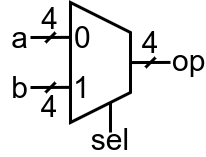
\includegraphics[width=0.40\textwidth]{img/04_vectors.png}
\end{figure}
\end{multicols}

\end{frame}

\note {
Ports, nets, and variables of the \textbf{reg} type are a single bit unless we declare them with a range.
\newline

To declare u multiple bit \textbf{port, net,} or \textbf{reg} variable, we need to specify a range. The range provides addresses for the individual bits. The only restriction on the range bounds is that they must be constant expressions. Either or both bound can be negative, zero, or positive, and the range can be ascending or descending.

}

%%%%%%%%%%%%%%%%%%%%%%%%%%%%%%%%%%%%%%%%%%%%%%%%%%%%%%%%%%%%
\begin{frame}
\frametitle{Using Vector Ranges}

Access vector selections whatever way you declared the range.
\begin{itemize}
\item Select one or more contiguous bits.
\end{itemize}
\begin{figure}[H!]
    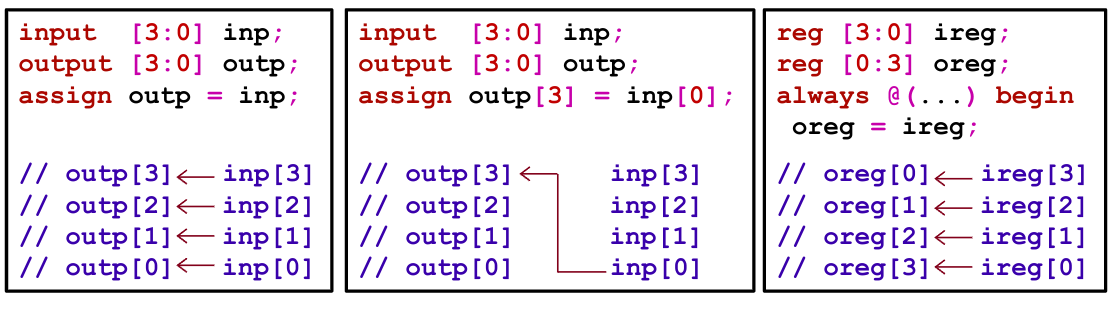
\includegraphics[width=0.95\textwidth]{img/04_range.png}
\end{figure}

\end{frame}

\note{
The vector range provides addresses for the individual bits. We can address a vector bit by providing an index and a vector part by providing a range. 
\newline

The part selection range must be in the same order as in the declaration, either ascending or descending.
\newline

The first illustration assigns an \textit{input} port to the \textit{output} port.
\newline 

The second illustration assigns one bit of an \textit{input} port to one bit of the \textit{output} port.
\newline

The third illustration assigns the value of a \textit{reg} vector to another \textit{reg} vector.

}

%%%%%%%%%%%%%%%%%%%%%%%%%%%%%%%%%%%%%%%%%%%%%%%%%%%%%%%%%%%%
\begin{frame}
\frametitle{Assigning Between Different Widths}
Vector widths do not need to match in an assignment!
\begin{itemize}
\item Source wider than target truncates value from msb.
\item Unsigned source shorter that target zero-extends value.
\item Signed source shorter that target sign-extends value.
\begin{itemize}
	\item Selections and concatenations are not considered signed.
\end{itemize}
\end{itemize}
\begin{figure}[H!]
    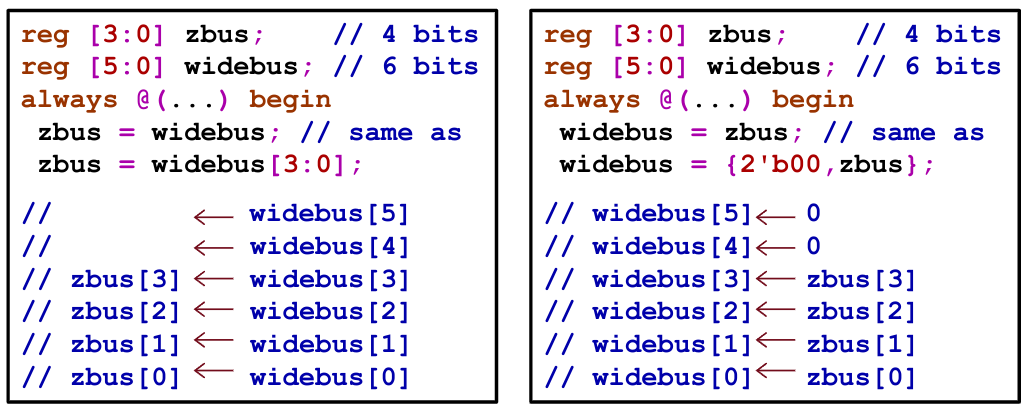
\includegraphics[width=0.95\textwidth]{img/04_width.png}
\end{figure}

\end{frame}

\note{
We can assign between vectors of different widths:
\begin{itemize}
\item Verilog truncates the leftmost bits when assigning a wider vector to a narrower vector. If we want to select some range other that the rightmost bits then you must specify that range.
\item Verilog pads the leftmost bits with 0 when assigning narrower vector to a wider vector. If you want to assign something other that 0, then you need to use the concatenation operator to construct a wider expression.
\end{itemize}
}
%%%%%%%%%%%%%%%%%%%%%%%%%%%%%%%%%%%%%%%%%%%%%%%%%%%%%%%%%%%%
\begin{frame}
\frametitle{Defining Literal Values}

We can specify a literal value as: \textcolor{red}{$<size>'<base><value>$}
\begin{itemize}
\item \textcolor{purple}{size} is an optional positive decimal number. If unsized is at least 32 bits.
\item \textcolor{purple}{base} is a character to indicate binary, octal, decimal, or hexadecimal radix.
\begin{itemize}
	\item B/b, O/o, D/d, H/h
	\item Verilog-2001: Optionally preceded by and "s" character to indicate a signed value.
\end{itemize} 
\item \textcolor{purple}{value} is legal digits for base:
\begin{itemize}
	\item Can include "\_" if not 1st character
	\item Can include Z/z and X/x if base is binary, octal or hexadecimal
	\item Verilog-2001: can be single Z/z or X/x digit if decimal base
	\item value is itself an unsigned number
\end{itemize}
\end{itemize}

\begin{figure}[H!]
    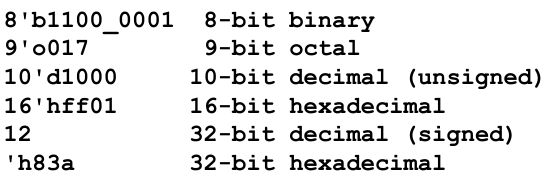
\includegraphics[width=0.55\textwidth]{img/04_literal.png}
\end{figure}

\end{frame}

\note{
\tiny{
We specify integer literals in binary, octal, decimal or hexadecimal format.
\newline

We can specify a decimal integer literal as an optional sign fallowed by a sequence of decimal digits. A number in this format is a signed number.
\newline

We can specify any integer literal as an optional sign fallowed by and optional size followed by a single quote followed by one or two base format characters and then followed by a sequence of digits appropriate to the radix.
\newline

A literal that we do not size has a size of at least 32 bits and most implementations make it exactly 32 bits.
\newline

There must be no white space between the single quote character and the base format. The base format is not sensitive to character case and consists of a \textbf{b, o, d, h} characters to indicate the radix.
\newline

The Verilog-2001 update allows an optional preceding "s" character to indicate a signed value.
\newline

The digit sequence is not sensitive to character case and consists of digits  for the radix. For the binary, octal or hexadecimal radices, we can use the "z" and "x" characters for any of the digits. The Verilog-2001 update also permits a decimal value to be a single "z" or "x" character to indicate a value that is high impedance or all unknown.
\newline

Except for the first digit, we can insert underscore "\_" characters anywhere we nedd them to improve readability. 
\newline

We can substitute the "?" character for a "z" character. This will become obvious when we study the case statement.
\newline

\textcolor{red}* Appropriately sizing the literal avoids padding and truncation!

}
}

%%%%%%%%%%%%%%%%%%%%%%%%%%%%%%%%%%%%%%%%%%%%%%%%%%%%%%%%%%%%
\begin{frame}
\frametitle{Automatic Extension of Unsigned Literals}
\scriptsize{
For \textcolor{purple}{sized literals} (e.g. 2'b11):
\begin{itemize}
\item Verilog pads to left with 0 to match size of wider expression.
\end{itemize}

For \textcolor{purple}{unsized literals} (e.g. 'b11):
\begin{itemize}
\item Size is 32 bits.
\item If leftmost digit is 1 or 0: 
\begin{itemize}
\scriptsize{
	\item Verilog left-fills to make 32 bits and pads to left with 0 to match the size of wider expression.
}
\end{itemize}
\item If leftmost digit is Z or X:
\begin{itemize}
\scriptsize{
	\item Verilog left-fills with that leftmost digit to make 32 bits.
	\item Verilog-1995 then pads to left with 0 to match size of wider expression.
	\item Verilog-2001: then pads to left with that leftmost digit to match size of wider expression.
}
\end{itemize}
\end{itemize}
}

\begin{multicols}{2}

\begin{figure}
    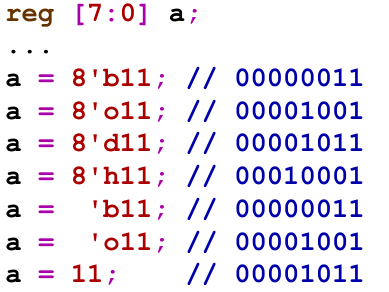
\includegraphics[width=0.35\textwidth]{img/04_ext0.png}
\end{figure}
\vfill

\columnbreak

\begin{figure}
    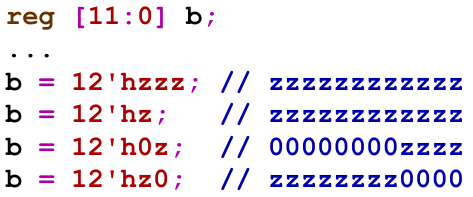
\includegraphics[width=0.45\textwidth]{img/04_ext1.png}
\end{figure}
\end{multicols}

\end{frame}

\note{
The Verilog 2001 standard permits signed based literals. The sign bit can be 0, 1, x or z. Verilog 2001 sign-extends signed based literals to match the width of the enclosing expression.
\newline

Verilog zero-extends unsigned based literals except in one situation. If the provided value has fever digits than what the size indicates and the leftmost bit is z or x, then Verilog extends the provided value with that z or x bit value up to the size of the literal. This made it easy to fill an entire vector with z or x.
\newline

The standard guarantees that the size of an unsigned literal is at least 32 bits and most implementations made it exactly 32 bits. The Verilog-2001 update continues to extend the z or x up to the width of the enclosing expression.

}

%%%%%%%%%%%%%%%%%%%%%%%%%%%%%%%%%%%%%%%%%%%%%%%%%%%%%%%%%%%%
\begin{frame}
\frametitle{Variable Vector Selection}
\begin{multicols}{2}
\scriptsize{
\textcolor{red}{Bit-select}:
\begin{itemize}
\item A single bit-select index may be variable.
\end{itemize}

\textcolor{red}{Range-select}:
\begin{itemize}
\item In Verilog-1995, range-select indices must be constant.
\item In Verilog-2001, a range-select can use a variable index and a constant width:
\begin{itemize}
\scriptsize{
	\item Base expression (variable)
	\item Width expression (constant)
	\item Offset direction:
	\begin{itemize}
		\scriptsize{
		\item Positive +
		\item Negative -
		}
	\end{itemize}
	\item Offset indicates if the width is added or substracted from the base:
}
\end{itemize}
\end{itemize}
}
\begin{figure}
    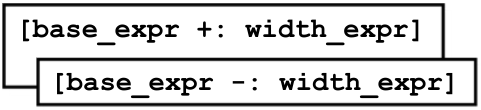
\includegraphics[width=0.45\textwidth]{img/04_offset.png}
\end{figure}
\vfill
\columnbreak

\begin{figure}
    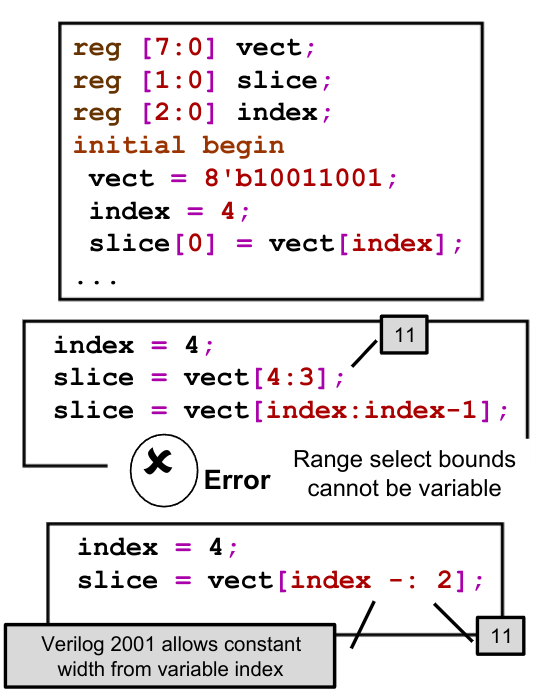
\includegraphics[width=0.45\textwidth]{img/04_selection.png}
\end{figure}
\end{multicols}

\end{frame}

\note{
\scriptsize{
Individual bits can be selected from a vector using a variable or expression index.
\newline

However in extracting a range of bits from a vector, Verilog-1995 requires that both bounds of the range are constants or constant expression. So a variable cannot be used in the extraction of a range of bits.
\newline

identifier {[msb\_constant\_expression:lsb\_constant\_expression]}
\newline

Verilog-2001 provides an alternative syntax that permits the starting point of a range select to be a variable expression, as long as the number of bits selected is a constant. In effect, to select a constant-width range from a variable starting bit position. The constant offset can be positive or negative from the starting point.
\newline

identifier {[base\_expression+:width\_constant\_expression]}
\newline
identifier {[base\_expression-:width\_constant\_expression]}
\newline

Where: \textit{base\_expression} is the variable starting bit position and \textit{width\_constant\_expression} is a constant plus or minus offset.

}
}

%%%%%%%%%%%%%%%%%%%%%%%%%%%%%%%%%%%%%%%%%%%%%%%%%%%%%%%%%%%%
\begin{frame}[fragile]
\frametitle{Declaring Nets}
\scriptsize{
\begin{multicols}{2}
Nets behave like physical wire. Values are driven onto them. Verilog has several net types.
Most commonly used is \textbf{wire}.

Verilog implicitly declares wires:
\begin{itemize}
\item Verilog-1995: Undeclared identifiers connected to instance ports.
\item Verilog-2001: Also undeclared identifier driven by continuous assignment.
\item Continuous assignments and instance output/inout ports drive nets.
\item Change default with compiler directive:
\begin{itemize}
\scriptsize{
	\item \begin{Verbatim}[commandchars=\\\{\}, tabsize=2]
\textcolor{blue}{`default_nettype <nettype>}
\end{Verbatim}
}
\end{itemize}
\end{itemize}
\vfill
\columnbreak

\begin{figure}
    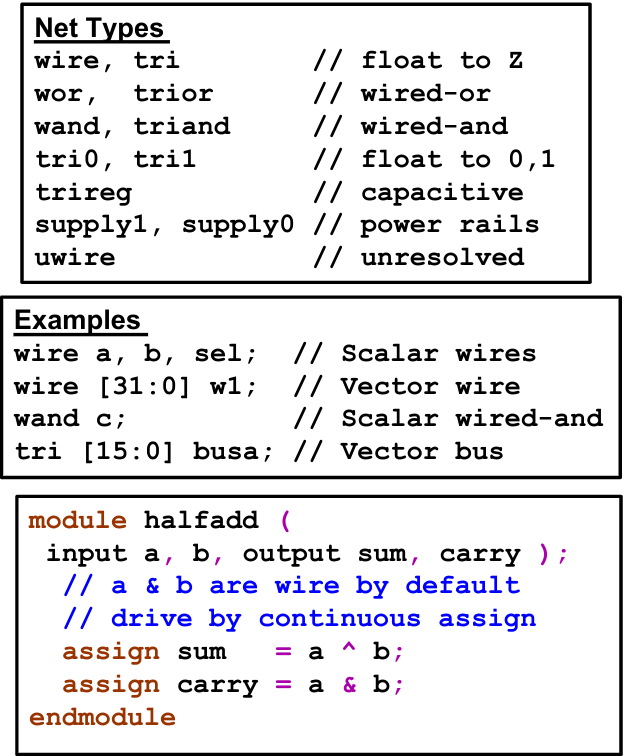
\includegraphics[width=0.45\textwidth]{img/04_declaring_nets.png}
\end{figure}
\end{multicols}
}
\end{frame}

\note{
\tiny{
Nets are continuously driven by their drivers. Verilog automatically propagates a new value onto a net when the drivers of the net change value. A net driver can be a continuous assignment or a module or primitive output.
\newline

Verilog has various net types for modeling design-specific and technology-specific functionality. The most common net type is a \textbf{wire}.
\newline

Verilog implicitly declares wire nets in some contexts in which you use a net without first declaring it. We can override this with compiler directive:
\begin{itemize}
\item \textbf{`defaul\_nettype} \textit{$<$nettype$>$}
\end{itemize}
With this directive, such undeclared nets default to the net type you specify in the compiler directive. For this directive, Verilog-2001 adds the \textit{none} net type. In other words, this doesn't allow implicit net declarations.
\newline

\textbf{net Types Functionality}
\begin{itemize}
\item wire, tri: For standard interconnection wires (default)
\item supply1: For power rails only in netlist
\item supply0: For ground rails only in netlist
\item wor, trior: For multiple drivers that are Wire-ORed
\item wand, triand: For multiple drivers that are Wier-ANDed
\item trireg: For nets with capacitive storage
\item tri0, tri1: For nets that pull up or down when not driven
\item uwire: Verilog-2005 unresolved wire accepts only one driver
\end{itemize}
}
}

%%%%%%%%%%%%%%%%%%%%%%%%%%%%%%%%%%%%%%%%%%%%%%%%%%%%%%%%%%%%
\begin{frame}[fragile]
\frametitle{Undeclared Identifier in Verilog}
\scriptsize{
A net is inferred for undeclared identifier by default in Verilog-2001. What's the issue?
\begin{itemize}
\item \textit{svm} is undeclared, so defaults to a single bit wire (implicit wire)
\item No compilation error/warning message
\item \textit{sum} output port is undriven as so becomes value Z
\item Mistyped identifier defaults to net/wire
\end{itemize}
What  is the solution?
\begin{itemize}
\item Check simulation carefully!
\item Write self-checking simulations
\item Use Verilog-2001 \begin{Verbatim}[commandchars=\\\{\}, tabsize=2]
\textcolor{blue}{`default_nettype <nettype>}
\end{Verbatim}
\end{itemize}
}
\begin{figure}
    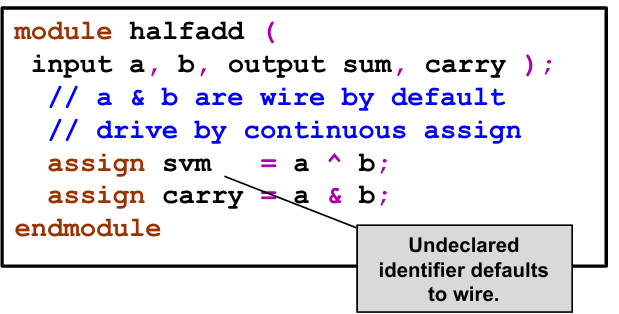
\includegraphics[width=0.55\textwidth]{img/04_typo.png}
\end{figure}
\end{frame}
\note{

Along with type, even lower-case and upper-case identifiers (user-defined name of some such as the module, wire, variable, or the name of the function) are perceived as different in Verilog. If an identifier is typed in upper-case by mistake, and is used on the left-hand side of a continuous assignment, then an implicit net declaration is inferred, and no error or warning is reported.
\newline

No error/warning is reported if undeclared identifier is used for connecting an instance of a module (this makes design debug difficult).
\newline

For the compiler directive \textbf{`defaul\_nettype} \textit{$<$nettype$>$}, Verilog-2001 adds the \textit{none} net type for compiler directive. In other words, this doesn't allow any implicit net declarations.

}


%%%%%%%%%%%%%%%%%%%%%%%%%%%%%%%%%%%%%%%%%%%%%%%%%%%%%%%%%%%%
\begin{frame}[fragile]
\frametitle{Usage of: \textbf{`default\_nettype} \textit{$<$nettype$>$}}
\footnotesize{
\begin{itemize}
\item Implicit wires can be avoided by using the \textcolor{red}{`default\_nettype none} compiler directive.
\item Any undeclared identifier is a compilation error/warning when this directive is used.
\item Directive can affect the compilation of other files once turned on.
\begin{figure}
    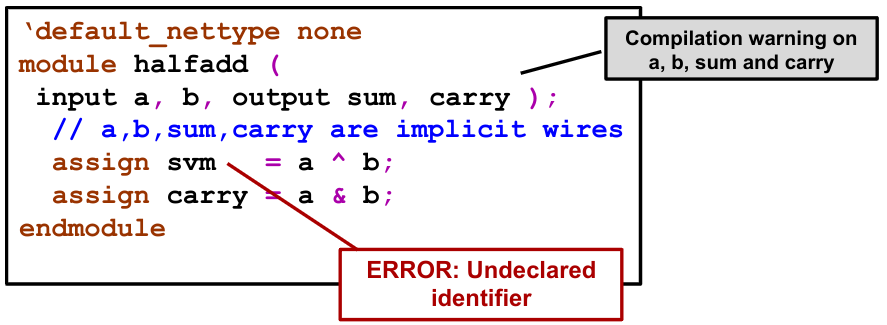
\includegraphics[width=0.85\textwidth]{img/04_none.png}
\end{figure}
\item Explicit declaration of identifier type is needed to avoid the error. This can be: \newline
\textcolor{red}{input wire a,b, output wire sum, carry}
\end{itemize}
}
\end{frame}

\note{
When \textbf{`default\_nettype none} compiler directive  is used, implicit data types are disabled. This can make any undeclared identifier name a syntax error. Hence, as a limitation of this directive, benefits of implicit data types are lost. Another limitation is that once this directive is turned on in one file, then the compilation of other files gets affected. To avoid this, the directive \textbf{`default\_nettype wire} should be added at the end of each file where implicit nets have been turned off.

}


%%%%%%%%%%%%%%%%%%%%%%%%%%%%%%%%%%%%%%%%%%%%%%%%%%%%%%%%%%%%
\begin{frame}
\frametitle{Merging Net Declaration and Assignment}
We can merge the net declaration and assignment - known as "net declaration assignment".
\begin{multicols}{2}
\begin{figure}
    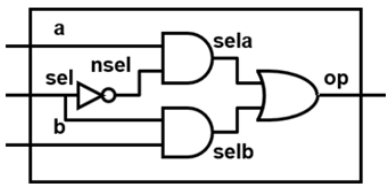
\includegraphics[width=0.35\textwidth]{img/04_merge.png}
\end{figure}
\vfill
\columnbreak

\begin{figure}
    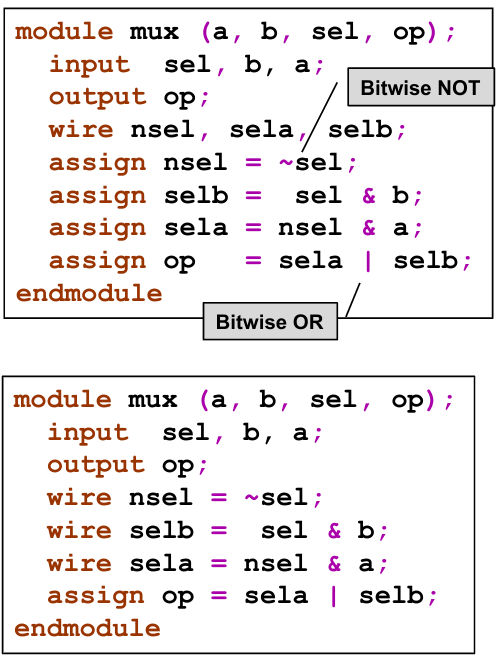
\includegraphics[width=0.45\textwidth]{img/04_merge_code.png}
\end{figure}
\end{multicols}
\end{frame}

\note{
We can merge the net declaration with an assignment to make a \textit{net declaration assignment}.
\newline

The first example explicitly declares the wires \textbf{nsel, nsela, nselb} and later makes continuous assignments to them.
\newline

The second example merges the wire declaration with a continuous assignment. We can still make additional continuous assignments to the nets. Remember that a net can have multiple drivers.
\newline

Ports that we do not declare otherwise are by default single-bit wire nets. Both examples also show a continuous assignment to the output port wire net.

}


%%%%%%%%%%%%%%%%%%%%%%%%%%%%%%%%%%%%%%%%%%%%%%%%%%%%%%%%%%%%
\begin{frame}[fragile]
\frametitle{Resolving Multiple Drivers of a Net}

\scriptsize{
\begin{multicols}{2}
\begin{itemize}
\item Multiple drivers can drive a net.
\item Exception is Verilog-2005 \textbf{uwire}.
\item Only a net can resolve the value of multiple drivers.
\end{itemize}

\vfill
\columnbreak
\begin{figure}
    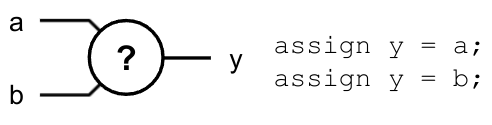
\includegraphics[width=0.45\textwidth]{img/04_multiple.png}
\end{figure}
\end{multicols}
\vfill
\begin{multicols}{3}
Two names - same type
\begin{Verbatim}[commandchars=\\\{\}, tabsize=4]
	wire y;
	tri y;
\end{Verbatim}
\vfill
\begin{figure}
    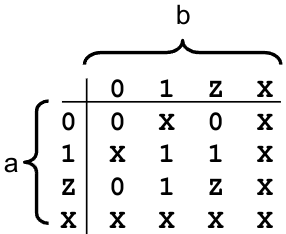
\includegraphics[width=0.3\textwidth]{img/04_multiple0.png}
\end{figure}

\vfill
\columnbreak
Two names - same type
\begin{Verbatim}[commandchars=\\\{\}, tabsize=4]
	wand y;
	triand y;
\end{Verbatim}
\vfill
\begin{figure}
    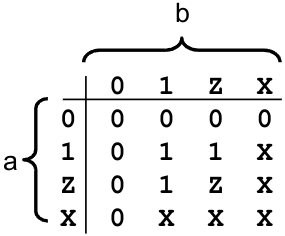
\includegraphics[width=0.3\textwidth]{img/04_multiple1.png}
\end{figure}

\vfill
\columnbreak
Two names - same type
\begin{Verbatim}[commandchars=\\\{\}, tabsize=4]
	wor y;
	trior y;
\end{Verbatim}
\vfill
\begin{figure}
    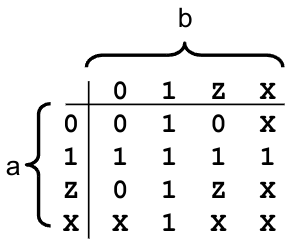
\includegraphics[width=0.3\textwidth]{img/04_multiple2.png}
\end{figure}
\end{multicols}
}
\end{frame}

\note{
\tiny{
Verilog resolves the value of a net driven by multiple drivers. Assuming that the drivers all have the same strength:
\begin{itemize}
\item The conflict of 0 and 1 values on a \textbf{wire} net results in an unknown value.
\item The conflict of 0 and 1 values on a wired-logic net results in a either 0 or a 1 value.
\end{itemize}

The \textbf{wire}, wired-and \textbf{wand}, and wired-or \textbf{wor} net types have two names. We can alternatively refer to them as \textbf{tri, triand} and \textbf{trior} types, respectively.
\newline

Net types \textbf{wire} and \textbf{tri} have identical functionality. They can be used in different names for better readability. That is, \textbf{tri} can be used in places when multiple drivers are present. Urban legend claims that the "tri" name exists to remind the user that they can assign high-impedance values to these nets. The urban legend neglects to explain the \textbf{tri0, tri1} and \textbf{trireg} nets that cannot have high-impedance value.
\newline

The wired-logic nets exist to model technology dependent logic conflict resolution:

\begin{itemize}
\item The wired-AND net to model open collector logic
\item The wired-OR net to model emitter coupled logic
\end{itemize}

Verilog-2005 added the \textbf{uwire} net type, an unresolved wire that allows no more than one driver. For Cadence INCISIV simulator, the \textit{uwire} needs the -sv switch.

}
}


%%%%%%%%%%%%%%%%%%%%%%%%%%%%%%%%%%%%%%%%%%%%%%%%%%%%%%%%%%%%
\begin{frame}
\frametitle{Declaring Variables}
\scriptsize{
Variables hold values that you procedurally assign. They keep the value until you assign a different value.
\begin{itemize}
\item \textbf{reg}: 4-state unsigned 1-bit
\begin{itemize}
	\item Can declare multi-bit vector
	\item Verilog-2001 adds \textbf{reg signed}
\end{itemize}
\item \textbf{integer}: 4-state signed 32-bit
\item \textbf{time}: 4-state unsigned 64-bit
\item \textbf{real}: Double precision float
\item \textbf{realtime}: Same as real
\end{itemize}
}

\begin{multicols}{2}
\begin{figure}
    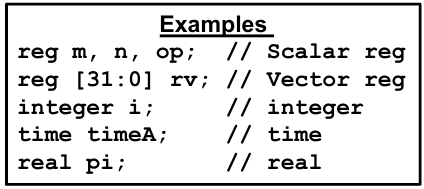
\includegraphics[width=0.45\textwidth]{img/04_var0.png}
\end{figure}
\vfill
\columnbreak

\begin{figure}
    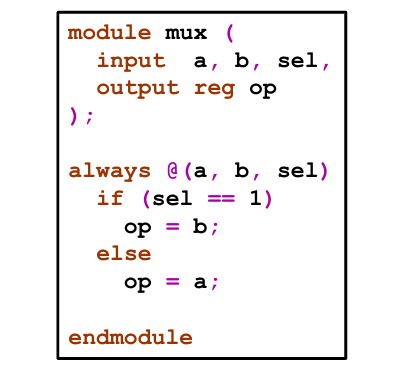
\includegraphics[width=0.45\textwidth]{img/04_var1.png}
\end{figure}
\end{multicols}
\end{frame}

\note{
\scriptsize{
A variable retains its value until we assign a new value to it.
\begin{itemize}
\item The \textbf{reg} type holds a four-state integral value. A \textit{reg} is by default unsigned but with Verilog-2001 update we can declare it signed. Arithmetic operations treat the value of a signed \textit{reg} as a signed value. A \textit{reg} is by default single bit wire, but we can declare an arbitrary range for it. The \textit{reg} is the most common variable type for hardware design.
\item The \textbf{integer} type holds a four-state signed integral value. The standard guarantees it to be at least 32 bits and most implementations make it exactly 32 bits. Arithmetic operations treat the value of an \textit{integer} as a signed value.
\item The \textbf{time} type holds a four-state unsigned integral value. The standard guarantees it to be at least 64 bits and most implementations make it exactly 64 bits. A \textit{time} is always unsigned. It is exactly the same as a 64-bit unsigned \textit{reg} vector. People typically use variables of this type to hold simulation time values.
\item The \textbf{real} type holds a double-precision floating-point value as described by IEEE Std 754-1985 Binary Floating-Point Arithmetic.
\item The \textbf{realtime} type is another name for \textit{real}. If we use it that way, we can use a \textit{realtime} to remind ourselves that its value is a real version of the simulation time.
\end{itemize}

}
}
%%%%%%%%%%%%%%%%%%%%%%%%%%%%%%%%%%%%%%%%%%%%%%%%%%%%%%%%%%%%
\begin{frame}
\frametitle{Making Assignments to Variables}
\begin{itemize}
\item We read a variable's value from inside or outside a procedure.
\item We write a variable's value only from inside a procedure.
\item Within a procedure we write only to variables.
\end{itemize}


\begin{multicols}{2}
\begin{figure}
    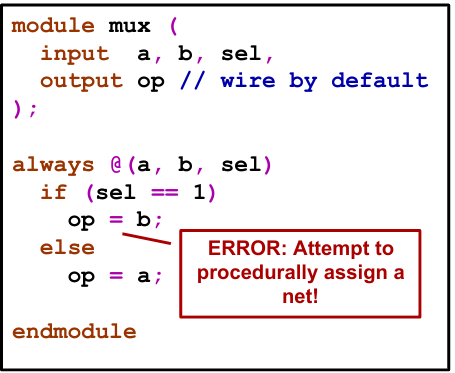
\includegraphics[width=0.45\textwidth]{img/04_vars0.png}
\end{figure}
\vfill
\columnbreak

\begin{figure}
    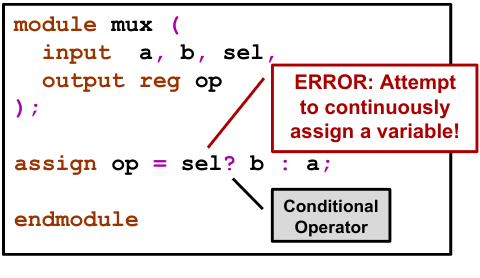
\includegraphics[width=0.45\textwidth]{img/04_vars1.png}
\end{figure}
\end{multicols}

\end{frame}

\note{
A variable can appear anywhere that we read its value.
\newline

Assignments to variables are procedural assignments. They exist only as a procedural statement.
\newline

The first example erroneously attempts to make a procedural assignment to a net. Remember that a port is implicitly declared as a single bit net unless we declare it otherwise.
\newline

The second example explicitly declares the port to be a \textbf{reg}, but then erroneously attempts to make a continuous assignment to the variable.

}
%%%%%%%%%%%%%%%%%%%%%%%%%%%%%%%%%%%%%%%%%%%%%%%%%%%%%%%%%%%%
\begin{frame}
\frametitle{Assigning Between Integers and Vectors}
\footnotesize{
\textbf{Reminder}
\begin{itemize}
\item \textbf{reg}: 4-state unsigned 1-bit
\begin{itemize}
\footnotesize{
	\item Can declare multi-bit vector
	\item Verilog-2001 adds \textbf{reg signed}
}
\end{itemize}
\item \textbf{integer}: 4-state signed 32-bit
\end{itemize}

Assignment between \textbf{reg} and \textbf{integer} follows previous rules:
\begin{itemize}
\item If value wider than target: Truncates value
\item If value shorter than target:
\begin{itemize}
\footnotesize{
	\item If unsigned value: zero-extends
	\item If signed value: sign-extends
}
\end{itemize}
\end{itemize}
}

\begin{figure}
    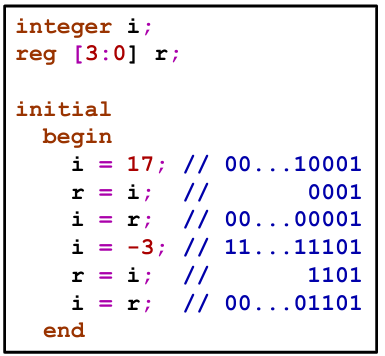
\includegraphics[width=0.35\textwidth]{img/04_int2reg.png}
\end{figure}
\end{frame}

\note{
\scriptsize{
We saw previously that Verilog truncates wide literal constants to fit shorter target widths and extends shorter literal constants to fit wider target widths, extending unsigned values with zero and signed values with sign bit. This is exactly the case also for assignments between \textit{integers} and \textit{vector reg} variables.
\newline

This example assigns the value 17 to an integer variable and assigns the integer to a 4-bit unsigned vector \textit{reg} variable. The assignment is a bit-for-bit replacement, so the vector \textit{reg} variable gets the value 1. Upon assigning the value of vector \textit{reg} variable to the integer variable, Verilog first zero-extends the value to match the width of the \textit{integer} variable, which is almost always 32 bits.
\newline

The example then assigns the value -3 to the integer variable and assigns the integer to the 4-bit vector \textit{reg} variable. The assignment is a bit-for-bit replacement, so the unsigned vector \textit{reg} variable gets the value 13. The sign is lost. Upon assigning the value of the vector \textit{reg} variable to the integer variable, Verilog zero-extends the value to match the width of the integer variable.

}
}

%%%%%%%%%%%%%%%%%%%%%%%%%%%%%%%%%%%%%%%%%%%%%%%%%%%%%%%%%%%%
\begin{frame}
\frametitle{Declaring Arrays of Nets and Variables}
\scriptsize{
Verilog-1995 supports one-dimensional arrays of \textbf{integer}, \textbf{reg} and \textbf{time}.
\begin{figure}
    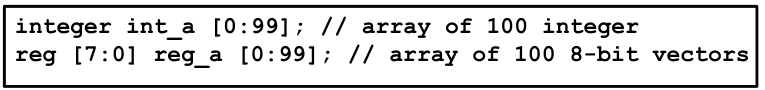
\includegraphics[width=0.85\textwidth, left]{img/04_array0.png}
\end{figure}

\begin{itemize}
\item We access one element (word) at a time by indexing to that word.
\item We cannot directly take bit or par selects of a word (use an intermediate variable)
\end{itemize}
\begin{figure}
    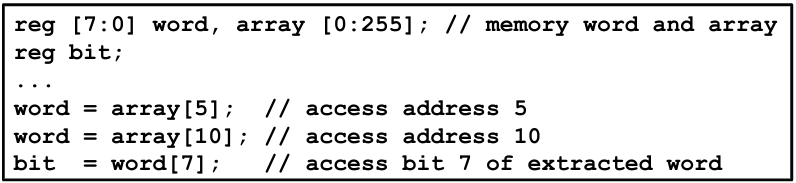
\includegraphics[width=0.85\textwidth, left]{img/04_array1.png}
\end{figure}

Verilog-2001 supports multi-dimensional arrays of \textbf{integer}, \textbf{real}, \textbf{realtime}, \textbf{reg}, \textbf{time} and \textbf{nets}.
\begin{figure}
    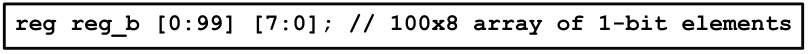
\includegraphics[width=0.85\textwidth, left]{img/04_array2.png}
\end{figure}
\begin{itemize}
\item We can directly take bit and part selects of an indexed element
\end{itemize}
\begin{figure}
    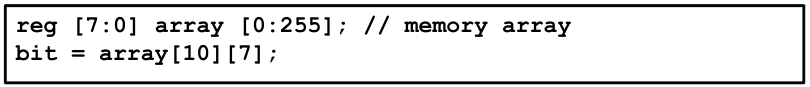
\includegraphics[width=0.85\textwidth, left]{img/04_array3.png}
\end{figure}
}
\end{frame}

\note{
\footnotesize{
As with programming languages, Verilog supports arrays:
\begin{itemize}
\item The Verilog-1995 standard permits one-dimensional arrays of \textbf{integer}, \textbf{reg} and \textbf{time}. The \textit{reg} elements can be either single-bit elements or vector \textit{reg} elements. People refer to an array of vector \textit{reg} elements as a Verilog "memory". The Verilog-2001 standard supports arrays of \textbf{integer, time, reg, real, realtime} and even \textbf{nets}, and they can have any number of dimensions.
\item The Verilog-1995 standard did not accommodate directly taking a bit-select or a part-select of an indexed memory element. We had to extract the element to a variable and then take a bit-select or part-select of the variable. The Verilog-2001 standard accommodate directly taking bit-select or a part-select of an indexed memory element.
\end{itemize}

}
}


%%%%%%%%%%%%%%%%%%%%%%%%%%%%%%%%%%%%%%%%%%%%%%%%%%%%%%%%%%%%
\begin{frame}
\frametitle{Declaring Module Parameters}
\begin{multicols}{2}

A module \textcolor{purple}{parameter} is an instance specific constant:
\footnotesize{
\begin{itemize}
\item Parametrizes the module definition (width, depth, frequency, time, etc.)
\item Can override for each individual instance 
\end{itemize}
}
\vfill
\begin{figure}
    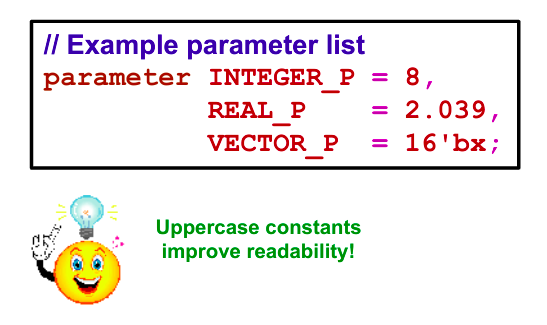
\includegraphics[width=0.45\textwidth]{img/04_param0.png}
\end{figure}
\columnbreak

\begin{figure}
    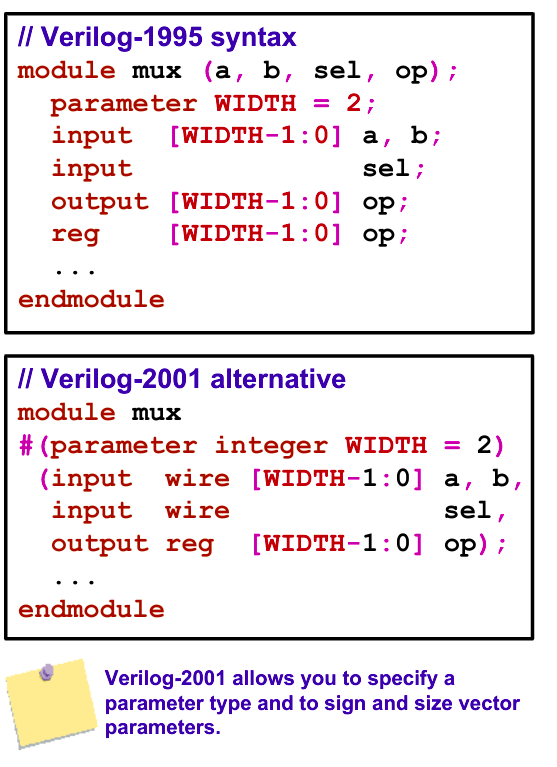
\includegraphics[width=0.45\textwidth]{img/04_param1.png}
\end{figure}

\end{multicols}
\end{frame}

\note{
\scriptsize{
Module parameters that we declare with \textit{parameter} keyword are constants that we can change for each instance of the module, thus we can use them to "parametrize" the instance, for example, to establish different widths and depths for each instance of a memory module. Parameters are not variables, so we cannot change them during simulation run time.
\newline

The first example on the slide uses the Verilog-1995 \textit{list of ports} syntax and declares the ports later as a module item. Before declaring ports, t declares a module parameter to establish the port width and sets the parameter's default value to 2. We can modify this parameter for each individual instance of the module.
\newline

The second example uses the Verilog-2001 \textit{list of port declarations} syntax. The example needs to declare the parameter before ports because it uses the parameter value to establish port width. It declares the parameter using the Verilog-2001 \textit{module parameter port list} syntax.
\newline

The Verilog-1995 syntax does not require a type declaration for a parameter - the parameter assumes the type of its initial value and we can change its type upon module instantiation by providing it a value of a different type. The Verilog-2001 syntax permits a type declaration for a parameter and any new value we provide must be of that type.

}
}

%%%%%%%%%%%%%%%%%%%%%%%%%%%%%%%%%%%%%%%%%%%%%%%%%%%%%%%%%%%%
\begin{frame}
\frametitle{Local parameters and Parameter Passing}

\scriptsize{
\begin{multicols}{2}
Localparams are true constants. unlike parameters, localarams cannot be overridden from the next level of hierarchy.
\newline

Use of constants that should never be overridden upon instantiation:
\begin{itemize}
\item For a module that is not instantiated (testbench?)
\item For "enumerations" (FSM states?)
\end{itemize}
Verilog-2001 provides three ways to override module parameters:
\begin{itemize}
\item Redefinition using \textbf{defparam}
\item Positional parameter override during instantiation
\item Named parameter override during instantiation (new in Verilog-2001)
\end{itemize}
\textcolor{red}* Parameter override using defparam can be difficult to track

\columnbreak

\begin{figure}
    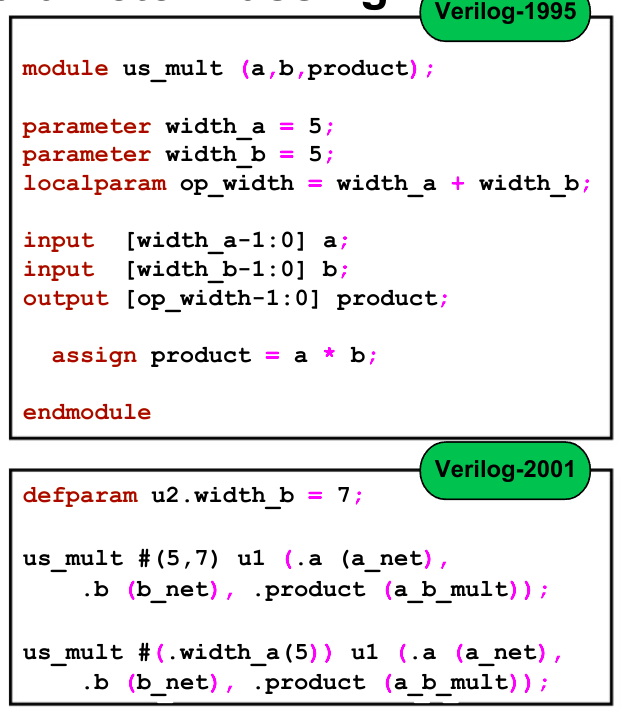
\includegraphics[width=0.45\textwidth]{img/04_param2.png}
\end{figure}

\end{multicols}
}
\end{frame}

\note{
\tiny{
The Verilog-2001 update provides the \textbf{localparam} construct - exactly like a parameter except that we cannon change it. For a module parameter that should not change on a per-module basis, we should use the \textit{localparam} keyword instead of the \textit{parameter} keyword.
\newline

To modify the parameters of a module instance, we can make a \textit{parameter value assignment} upon instantiating the module. A parameter value assignment is a parenthesized list of parameter assignments before the module instance name and prefixed with a hash ("\#") character. We may see the hash character used in other context to specify propagation delay, but in the context of a module instantiation, it is a parameter value assignment or parameter value override during instantiation.
\newline

Out list of parameter assignments can use either the Verilog-1995 ordered parameter assignment syntax or the Verilog-2001 named parameter assignment syntax, but we cannot mix the two syntaxes in the same instantiation. These syntaxes are similar to the ordered and named port connection syntax, but with the ordered parameter assignment syntax, we cannot merely insert a comma as a place holder - we need to provide values for all earlier parameters of we want to provide a value for a later parameter. This example uses the ordered parameter assignment syntax, but we should in general use the named parameter assignment syntax to make our code more readable.
\newline

We can also override a parameter value by using \textbf{defparam} statement. A parameter can be modified using the \textit{defparam} statement during compilation time. We can make this override from anywhere in the design by using a hierarchical parameter name. Our use of this override is superfluous when done locally and can potentially cause much confusion when not done locally as it might be difficult to track.
\newline

\textit{localparam} cannot be directly modified by \textit{defparam} statements. \textbf{Specparam} provides timing and delay values and can be modified through SDF annotation only (Refer appendix C for SDF annotation).

}
}
%%%%%%%%%%%%%%%%%%%%%%%%%%%%%%%%%%%%%%%%%%%%%%%%%%%%%%%%%%%%
\begin{frame}
\frametitle{Module Summary}
A net behaves like a physical wire driven by logic:
\begin{itemize}
\item Implicitly declared nets default to type wire
\item We drive nets by continuous assignments and by module and primitive outputs
\end{itemize}
A variable stores a value:
\begin{itemize}
\item We update a variable only by a procedural assignment
\item We make a procedural assignment only to a variable
\item Assignment between \textbf{integer} and \textbf{reg} ignore sign.
\end{itemize}
Expressions that read nets and variables can exist inside or outside procedures.
A module port we do not declare otherwise is implicitly declared \textbf{wire}.
\begin{itemize}
\item Input ports are nets driven externally by nets and/or variables.
\item Inout ports are nets connected externally to nets.
\item Output ports are nets or variables externally driving nets.
\end{itemize}
\end{frame}

\note{
This module examined the Verilog value set and data types. It explored nets, variables, and a form of a constant called a parameter.

}
%%%%%%%%%%%%%%%%%%%%%%%%%%%%%%%%%%%%%%%%%%%%%%%%%%%%%%%%%%%%
\begin{frame}
\frametitle{Module Review}
\begin{enumerate}
\item What are the four logic values in the Verilog value set?
\item Rewrite the binary value 8'b11010011 in hexadecimal.
\item How many bits wide is the integer type?
\item What is the primary difference between a net and a variable?
\end{enumerate}
\end{frame}

\note{
\begin{enumerate}
\item What are the four logic values in the Verilog value set?
\begin{itemize}
	\item 0 1 Z X
\end{itemize}
\item Rewrite the binary value 8'b11010011 in hexadecimal.
\begin{itemize}
	\item 8'hd3
\end{itemize}
\item How many bits wide is the integer type?
\begin{itemize}
	\item 32
\end{itemize}
\item What is the primary difference between a net and a variable?
\begin{itemize}
	\item A net is continuously driven, behaving like a physical wire driven by logic. A variable represents storage, storing a value until a new one is assigned. In the language, we can assign variables only from procedural statements and nets only from continuous assignments.
\end{itemize}
\end{enumerate}

}

%%%%%%%%%%%%%%%%%%%%%%%%%%%%%%%%%%%%%%%%%%%%%%%%%%%%%%%%%%%%
\begin{frame}
\frametitle{Module Exercise}
Code this two-input AND operation using a:
\begin{enumerate}
\item \textbf{wire}
\item \textbf{reg}
\end{enumerate}
\begin{figure}
    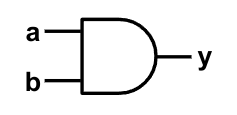
\includegraphics[width=0.25\textwidth]{img/04_exercise.png}
\end{figure}
\end{frame}

\note{
Solution:

\begin{figure}
    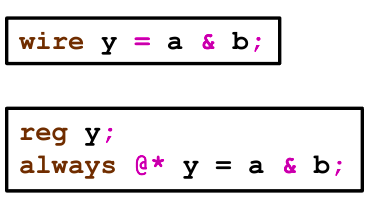
\includegraphics[width=0.25\textwidth]{img/04_exercise0.png}
\end{figure}
}

%%%%%%%%%%%%%%%%%%%%%%%%%%%%%%%%%%%%%%%%%%%%%%%%%%%%%%%%%%%%
\begin{frame}
\frametitle{Lab}
Lab 5-1: Modeling a Data Driver
\begin{itemize}
\item Use a Verilog literal value while describing a parametrized-width bus driver.
\end{itemize}

\begin{figure}
    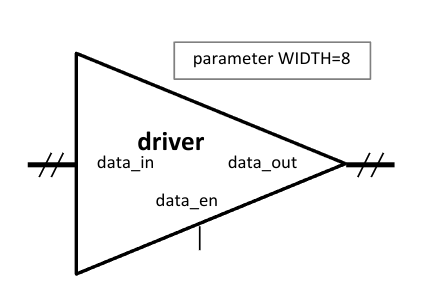
\includegraphics[width=0.35\textwidth]{img/04_lab.png}
\end{figure}
\end{frame}

%%%%%%%%%%%%%%%%%%%%%%%%%%%%%%%%%%%%%%%%%%%%%%%%%%%%%%%%%%%%
\begin{frame}
\frametitle{Test Your Understanding - 1}
The simulator reports a signal state as "X". This means that the signal state is:
\begin{itemize}
\item[$\square$] unknown
\item[$\square$] randomly both binary 0 and 1
\item[$\square$] high impedance
\item[$\square$] unresolved either binary 0 or 1
\end{itemize}
\end{frame}

\note{
The simulator reports a signal state as "X". This means that the signal state is:
\begin{itemize}
\item[$\boxtimes$] unknown
\item[$\square$] randomly both binary 0 and 1
\item[$\square$] high impedance
\item[$\square$] unresolved either binary 0 or 1
\end{itemize}

}


%%%%%%%%%%%%%%%%%%%%%%%%%%%%%%%%%%%%%%%%%%%%%%%%%%%%%%%%%%%%
\begin{frame}
\frametitle{Test Your Understanding - 2}
While describing our design we can use a range of net types including:
\begin{itemize}
\item[$\square$] pull1
\item[$\square$] tri1
\item[$\square$] trireg
\item[$\square$] triand
\item[$\square$] supply1
\item[$\square$] tri
\end{itemize}
\end{frame}

\note{
While describing our design we can use a range of net types including:
\begin{itemize}
\item[$\square$] pull1
\item[$\boxtimes$] tri1
\item[$\boxtimes$] trireg
\item[$\boxtimes$] triand
\item[$\boxtimes$] supply1
\item[$\boxtimes$] tri
\end{itemize}

}

%%%%%%%%%%%%%%%%%%%%%%%%%%%%%%%%%%%%%%%%%%%%%%%%%%%%%%%%%%%%
\begin{frame}
\frametitle{Test Your Understanding - 3}
We want to declare a 4-bit vector. Which range specification(s) can we use?
\begin{itemize}
\item[$\square$] {[0:3]}
\item[$\square$] {[3:0]}
\item[$\square$] {[1:4]}
\item[$\square$] {[4:1]}
\item[$\square$] {[2:-1]}
\item[$\square$] {[-1:2]}
\end{itemize}
\end{frame}

\note{
We want to declare a 4-bit vector. Which range specification(s) can we use?
\begin{itemize}
\item[$\boxtimes$] {[0:3]}
\item[$\boxtimes$] {[3:0]}
\item[$\boxtimes$] {[1:4]}
\item[$\boxtimes$] {[4:1]}
\item[$\boxtimes$] {[2:-1]}
\item[$\boxtimes$] {[-1:2]}
\end{itemize}

}

%%%%%%%%%%%%%%%%%%%%%%%%%%%%%%%%%%%%%%%%%%%%%%%%%%%%%%%%%%%%
\begin{frame}
\frametitle{Test Your Understanding - 4}
We have used an unsized integer literal in an expression. The elaborator inserts a value of a size that is at least:
\begin{itemize}
\item[$\square$] 32
\item[$\square$] 64
\item[$\square$] 16
\item[$\square$] 8
\end{itemize}
\end{frame}

\note{
We have used an unsized integer literal in an expression. The elaborator inserts a value of a size that is at least:
\begin{itemize}
\item[$\boxtimes$] 32
\item[$\square$] 64
\item[$\square$] 16
\item[$\square$] 8
\end{itemize}

}

%%%%%%%%%%%%%%%%%%%%%%%%%%%%%%%%%%%%%%%%%%%%%%%%%%%%%%%%%%%%
\begin{frame}
\frametitle{Test Your Understanding - 5}
We declared an inout port associated with an internal module item. We can make a procedural assignments to that item?
\begin{itemize}
\item[$\square$] True
\item[$\square$] False
\end{itemize}
\end{frame}

\note{
We declared an inout port associated with an internal module item. We can make a procedural assignments to that item?
\begin{itemize}
\item[$\square$] True
\item[$\boxtimes$] False
\end{itemize}

}

\end{document}
